\documentclass[12pt]{article}

\usepackage[utf8]{inputenc}
\usepackage{amsmath}
\usepackage{fancyhdr}
\usepackage{graphicx}
\usepackage{vmargin}
\usepackage{tikz}
\usepackage{pgfplots}

%%%%%%%%%%%%%%%%%%%%%%%%%%%%%%%%%%%%%%%%%%%%%%%%%%%%%%%%%%%%%%%%%%%%%%%%%%

\setmarginsrb{3 cm}{2.5 cm}{3 cm}{2.5 cm}{1 cm}{1.5 cm}{1 cm}{1.5 cm}
\pagestyle{fancy}
\fancyhf{}
\rhead{}
\chead{}
\lhead{}
\rfoot{side \thepage}

\title{}
\author{}

%%%%%%%%%%%%%%%%%%%%%%%%%%%%%%%%%%%%%%%%%%%%%%%%%%%%%%%%%%%%%%%%%%%%%%%%%%

\begin{document}
\maketitle

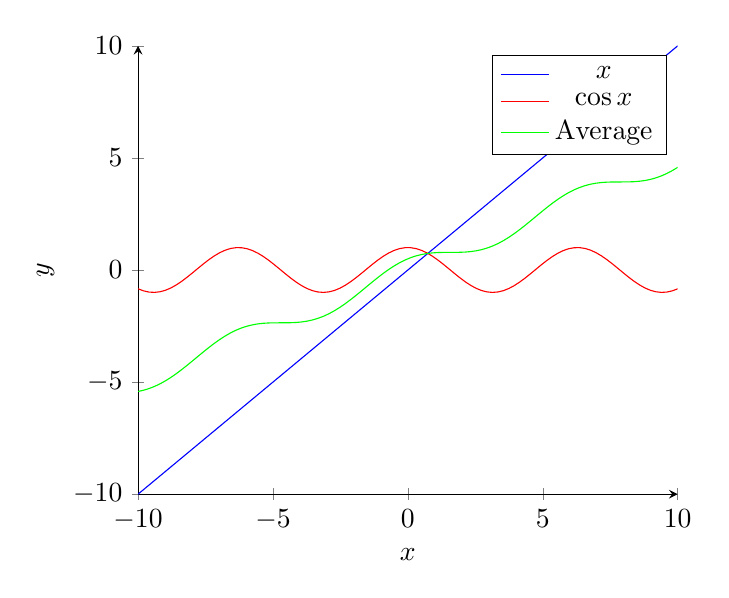
\begin{tikzpicture}
  \begin{axis}[
    axis lines = left,
    xlabel = $x$,
    ylabel = $y$,
    ]

    \addplot [
    domain = -10:10,
    samples = 100,
    color = blue,
    ]
    {x};
    \addlegendentry{$x$}

    \addplot [
    domain = -10:10,
    samples = 100,
    color = red,
    ]
    {cos(deg(x))};
    \addlegendentry{$\cos{x}$}

    \addplot [
    domain = -10:10,
    samples = 100,
    color = green,
    ]
    {(cos(deg(x))+x)/2};
    \addlegendentry{Average}
  \end{axis}
\end{tikzpicture}


\end{document}
